\chapter{Steepest Descent}
The Laplace and Stationary phase methods can be seen as the real and imaginary parts of the method of ``steepest descent''. Quick recap:
\begin{enumerate}
	\item The Laplace method is used to solve integrals that look like
	\begin{gather*}
		\int_{a}^{b} f(t) \me^{x \phi(t)} \md t \qquad x \rightarrow \infty 
	\end{gather*}
	and can give the whole asymptotic expansion. But needs $\phi(t)$ to be real and bell-shaped with the dominant contribution coming from the neighborhood of the peak as $x \rightarrow \infty$ (bell narrows). {\bf NB} We can write any $\phi(t) = 1+ \tau^2$ if its maxima exists in the domain of integration. Or else the dominant contribution should come from the boundary terms.  
	\item The Stationary phase method deals with integrals of the form
	\begin{gather*}
		\int_{a}^{b} f(t)\me^{\mi x \psi(t)} \md t \qquad x \rightarrow \infty 
	\end{gather*}
	This only gives us the leading term plus requires pure imaginary exponent. The rapid oscillations typically cancel except near the point of stationary phase, which provides the dominant contribution. The oscillations becomes more rapid with increasing $x$. 
\end{enumerate}
With the steepest descent method we can recover higher order terms cf. stationary phase method (improves and generalizes upon both methods). Consider
\begin{gather*}
	I(x) = \int_{a}^{b} h(t) \me^{x \rho(t)} \md t \qquad x \rightarrow \infty
\end{gather*}
where $\rho(t) = \phi(t) + \mi \psi(t)$ is an \emph{analytic function} and we perform the integral in the complex $t$ plane with $t=u + \mi v$. \\
\ \newline
\paragraph{Idea} We wish to deform the integral $\int_{a}^{b}$ from the real axis to a new contour $C$ on which $\Im [\rho(t)] = \psi(t)$ is constant! This constant can be different on different pieces of the contour. Then
\begin{align*}
	I(x) = \me^{\mi x \psi}\int_{a}^{b} h(t) \me^{x \phi(t)} \md t
\end{align*}
and the problem becomes amenable to Laplace's method. It is worth noting that the function $\phi(t)$ changes most rapidly along curves of constant $\psi(t)$ -- hence the name! This is illustrated through an example.

\paragraph{Example:} Consider 
\begin{align*}
	I(x) &= \int_{0}^{1} \me^{\mi x t^2} \md t \\
	&= \int_{0}^{1} \me^{\mi x (u^2-v^2)}\me^{- 2x u v} \md t
\end{align*}
We want to replace the current path with a new contour -- connecting the two end points -- such that $\psi = u^2-v^2$ is constant on each piece of the contour. Note that 
\begin{gather*}
	\psi(0,0) = 0 \qquad \psi(1,0) = 1
\end{gather*}
which means the contour must be broken up into at least two pieces. At the origin since $\psi = 0$, the stationary phase requires that $u=\pm v$. At $(1,0)$, we find $v = \pm \sqrt{u^2-1}$. 
\begin{figure}[h]
	\centering
	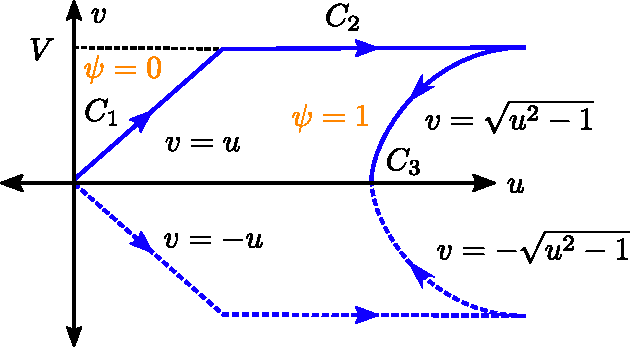
\includegraphics[width=0.66\textwidth]{./plots/pdf/steepestdescent.pdf}
	\caption{}
	\label{fig:strogatz-wk06}
\end{figure}\\
Let us see how $\phi(t)$ behaves on these pieces as we take the bridge to infinity (Fig. \ref{fig:strogatz-wk06}): 
\begin{enumerate}
	\item $C_1$: On $u=v$, $\psi=0$ and $\phi = -2v^2$. As $v$ runs from $0$ to $\infty$, the function decreases monotonically. This is good since the maximum value occurs at (0,0). If instead we chose $u=-v$, the function would have increased as we moved towards infinity, making it unwieldy and requiring careful cancellations of the infinities.
	\item $C_3$: On the $\psi = 1$ piece given by the hyperbola, $u = \sqrt{v^2+1}$. We see $\phi = -2v\sqrt{v^2+1}$ which peaks at $v=0$ and decreases as we move towards infinity. 
	\item On the bridge given by the contour $C_2$, $\psi$ is not constant. The contribution of this term is
	\begin{align*}
		\int_{C_2} \me^{-\mi x t^2} \md t &\leq \int_{C_2} \underbrace{| \me^{\mi x (u^2 - v^2)}|}_1|\me^{-2xuv}| \md t  \\
		& = \int_{u_1}^{u_2} \me^{-2xuV} \md u \rightarrow 0
	\end{align*}
	as $V \rightarrow 0$ and $x \rightarrow \infty $.
\end{enumerate}
Therefore
\begin{align*}
	I(x) &= (1+\mi)\int_0^\infty  \me^{-2xv^2} \md v + \me^{\mi x} \int_\infty^0  \me^{-2x v \sqrt{v^2+1}} \left[\frac{v}{\sqrt{v^2+1}}+\mi \right]\md v\\
	&= \frac{(1+\mi)}{2} \sqrt{\frac{\pi}{2x}} + \me^{\mi x} \int_{\infty}^{0} \me^{-2xv(1+\dots) }(\mi + \dots )\md v \\
	& \sim \frac{1}{2}\me^{\mi \pi/4} \sqrt{\frac{\pi}{x}} - \frac{\mi }{2x}\me^{\mi x}
\end{align*}
where in evaluating the second integral, we note that the integrand is sharply peaked about $v=0$ and is set up for Laplace's method. To the leading order, and most crudely, we have simply set $v=0$. \\
\ \newline
There is a neater way to find the integral along $C_3$: since the contribution is coming from the infinitesimal neighborhood of the maxima at $t=1$, we do not care about the full hyperbolic equation, instead approximate $C_3$ by its tangent line -- the detailed global shape of $C_3$ is irrelevant. So we can directly write
\begin{gather*}
	t = 1+ \mi v \qquad v \in [0,\epsilon)
\end{gather*}  
and
\begin{align*}
	I_3 = \int_{C_3} \me^{\mi xt^2} \md t &= \int_{\epsilon}^{0} \me^{\mi x (1+ \mi v)^2} \mi \md v \\
	&= -\mi \me^{\mi x}\int_{0}^{\infty} \me^{-2xv} \me^{-\mi x v^2}\md v \\
	&= -\mi \me^{\mi x} \int_{0}^{\infty} \me^{-2xv} \left[1 - \mi x v^2 + \dots\right] \md v \\
	& \sim -\frac{\mi }{2x}\me^{\mi x} \left[1 - \frac{\mi}{2x}\right]
\end{align*}

  
